\documentclass[12pt,letterpaper,fleqn]{article}
%%%%%%%%%%%%%%%%%%%%%%%%%%%%%%%%%%%%%%%%%%%%%%%%%%%%%%%%%%%%%%%%%%%%%%%%%%%%%%%%%%%%%%%%%%%%%%%%%%%%%%%%%%%%%%%%%%%%%%%%%%%%%%%%%%%%%%%%%%%%%%%%%%%%%%%%%%%%%%%%%%%%%%%%%%%%%%%%%%%%%%%%%%%%%%%%%%%%%%%%%%%%%%%%%%%%%%%%%%%%%%%%%%%%%%%%%%%%%%%%%%%%%%%%%%%%
\usepackage{amsfonts}
\usepackage{amsmath,amsthm,amssymb}
\usepackage{fullpage}
\usepackage{graphicx}
\usepackage{color}
\usepackage{caption}
\usepackage{subcaption}
\usepackage{times}
\usepackage[normalem]{ulem}
\usepackage{comment}
\usepackage{epsfig}
\usepackage{ascmac}
\usepackage{slidesec}

\newcommand{\gb}{\beta}
\newcommand{\gt}{\tau}
\newcommand{\gd}{\delta}
\newcommand{\gL}{\Lambda}
\newcommand{\gD}{\Delta}
\newcommand{\gl}{\lambda}
\newcommand{\gk}{\kappa}
\newcommand{\gs}{\sigma}
\newcommand{\hgs}{\hat{\sigma}}
\newcommand{\mcf}{\mathcal{F}}
\newcommand{\mcg}{\mathcal{G}}
\newcommand{\mch}{\mathcal{H}}
\newcommand{\mcs}{\mathcal{S}}
\newcommand{\mcr}{\mathcal{R}}
\newcommand{\hatm}{\hat{\mu}_i(\xi)}
\newcommand{\ga}{\alpha}
\newcommand{\gr}{\rho}
\newcommand{\mbf}{\mathbb{F}}
\newcommand{\mbg}{\mathbb{G}}
\newcommand{\mbh}{\mathbb{H}}
\newcommand{\mbq}{\mathbb{Q}}
\newcommand{\mbp}{\mathbb{P}}
\newcommand{\mbr}{\mathbb{R}}
\newcommand{\var}{\mbox{Var}}
\newcommand{\cov}{\mbox{Cov}}
\newcommand{\tp}{\tilde{p}}
\newcommand{\bp}{\bar{p}}
\setcounter{MaxMatrixCols}{10}

\newcommand{\mbn}{\mathbb{N}}
\newcommand{\bee}{\begin{equation}}
\newcommand{\eee}{\end{equation}}
\newcommand{\mcl}{\mathcal{L}}
%\newcommand{\gep}{\epsilon}
\newcommand{\raw}{\rightarrow}
\newcommand{\rawi}{\rightarrow\infty}
\newcommand{\mesh}{\text{mesh}}
\newcommand{\Om}{\Omega}
\newcommand{\gep}{\varepsilon}

\graphicspath{ {./Figures/} }
\begin{document}


\begin{center} {\Huge An algorithm for spike sorting with electrical artifact\bf\\ }
\vskip .2in {\Large\bf Gonzalo Mena, Lauren Grosberg, Liam Paninski and EJ Chichilnisky} \\
\today
\end{center}

\bigskip
\abstract{We developed an algorithm that successfully automatizes spike sorting with electrical artifact. In the following, the method is succinctly described and results are shown for 56 datasets from electrical stimulation experiments}
\section{Introduction}
In a retinal prosthetic context one is ultimately concerned with building probabilistic models of how cells responds to electrical activity. This can be thought in the same terms as in the neural coding problem, which is stated probabilistically : what is the probability of a response across a neural population given a particular natural stimulus (for example, an image)? \cite{paninski2004}. The difference is that the stimulus is now replaced by an artificial, electrical one. Whichever model is built, data is necessary for it's fitting and for subsequently providing a solution for the inverse decoding problem: how an electrical stimulatus has to be chosen int order to elicit an arbitrary response? Naturally, the most relevant information required for the fitting of any of such models is contained in the set of stimulus-response pairs, and whereas the stimulus is controlled by the experimenter, responses (spikes) have to be identified from electrode recordings. This problem, of distinguishing particular action potentials of neurons from extracellular voltage recordings, is known in the literature as spike sorting. In consequence, any framework for achieving controlled arbitrary responses in neurons via electrical stimulation will rely on spike sorting as a fundamental building block of its computational implementation. Because of the central importance of spike sorting in systems neuroscience, in the past decades many different methodologies have been developed for automatizing the detection of spikes, and significant improvements in accuracy and computational efficiency have been achieved\cite{LewickiSS,PillowShlens,Ekanadham201447,Rey2015}. However, the context of electrical stimulation constitutes a departure from the realm where current spike sorting methodologies apply, as the electrode recordings are now corrupted by the transient activity induced by this exogenous stimulation. This corruption or artifact can have an overwhelming impact in the recorded traces, making the spike identification process challenging even for of the human expert (see figure 1). Actually, previous to this work the only available spike sorting method relied heavily on human judgement, and because of the difficulty of telling spikes apart from the artifact, it was extremely time consuming even for datasets of modest size. In this article we provide the first scalable algorithmic approach for spike sorting in the presence of electrical stimulation artifact.


\subsection{Electrical artifact}
*LAUREN HAS THINGS TO SAY ABOUT THIS, WHICH ARE THE SOURCES OF THE ARTIFACT, TRIAL BY TRIAL VARIABILITY,  CHANGES IN TIME AND AMPLITUDE (INCLUDING BREAKPOINTS) DISTINCTION BETWEEN HARDWARE/AXON BUNDLE*
 The main problem is the presence of electrical artifact, which is a consequence of the electric field generated by the stimulation, and whose ubiquitous presence hampers the spike identification process. Actually, because of the electrical artifact, whose amplitude can be several times larger than of action potentials, spikes can become almost non-identifiable: suppose for example all trials at condition $j$ have spikes and there is little variability in spiking times. Suppose also the artifact is nearly the same across trials, so the recorded traces, assumed to be the artifact plus action potentials plus noise would look almost identical for all trials, and we may conclude that either there are no spikes at all, or that there are spikes at every trial (in which case, spiking times could be any). A more dramatic example corresponds to the situation where there is only one trial per condition. Then, spike sorting is impossible as there is no way to tell the artifact and action potential (if any) apart. The moral is that if we are completely agnostic about how artifact looks like there is little we can do. However, if we impose structure about how the artifact looks like and how often spikes should show up as a function of condition, then better chances are spikes will be identified better.   
\section{Methods}

As shown in figure 1,trial by trial spike identification can be impossible even if templates are available. An appropriate experimental design is crucial to allow the simultaneous inference of spikes and artifact. This design should exploit neurophisiological the overcome the identifiability issues
 \subsection{Data description}
%avoid redundancies with stimulation and change pattern
Suppose spike sorting is required for a set of $N$ neurons. Apart from the templates of these neurons, Data consists of a set of $I$ voltage traces, or trials, measured both across time ($t=1\ldots T$, corresponding to multiples of the sample rate) and a set of recording electrodes in the array ($e=1\ldots E$), as a response to electrical stimulation (although in principle there are as many as 512 electrodes, we only consider for subsequent analysis the ones where the spike waveform have a strong enough signal, that should correspond to nearby locations of the somas of neurons) These traces are organized into a design as follows: first, a number of $J$ different stimulus are chosen, defined by the current amplitudes of the pulses that are passed into a subset of electrodes in the array (that may or may not overlap with the recording electrodes). For separate datasets, references to specific currents and stimulating electrodes can be avoided, and replaced by the reference to the $j-th$ stimulus condition, since the stimulating electrodes remain the same and currents into each electrode always belong to the same line and increase monotonically with the index $j$. Then, for condition $j$, a number of $I_j$ traces are available. Thus,  $I = \sum_j I_j$. Naturally, templates of neurons for which spike sorting are required is done in 


\subsection{Assumptions}
In order to come up with a generative model for which we can do tractable inferences, some assumptions have to be made. Although they are simplifications, taken together they seem to provide reasonable enough account of the data. First, we assume that spikes, artifact and noise interact linearly, and thus the observed traces are the sum of these three components (HOW CAN WE JUSTIFY THIS). Regarding the noise terms, they are assumed gaussian and trial-to-trial independent, and their variances electrode and condition dependent, reflecting different responses of the background neural tissue (which are believed to be responsible of the observed noise) to different stimulus (figure). Also, noise processes are assumed uncorrelated in  in time and electrodes. This is certainly arguable: it is known that noise terms exhibit large both spatial and temporal correlations \cite{PillowShlens}, but if these correlations were explicitly accounted for by the model then different covariance matrices should be estimated, one per each condition $j$. This would entail a non negligible additional computational burden, but most importantly, would prescribe the gathering of larger number of trials to allow reliable estimation of such matrices. As results with synthetic data created from the projection of real data on the simplified model shows that results are essentially the same regardless the correlations, and because in the first applications of this method we will deal with rather simple cases where noise correlations should not be a major issue, we prefer to maintain this assumption. Regarding the artifact, we assume it is a function of time and condition $j$, but remains the same for different trials. This comes from voltage recordings in TTX experiments, where no neural driven activity is expected to occur, and where it is observed that trial-to-trials variations in the traces within the same condition are well explained by the noise. The Artifact is also assumed to possess a regularized structure: both variations in time and condition (see TTX figure) are assumed smooth. Regarding activity of neurons for which we do spike sorting, we assume a set of $N$ spike templates are available , each of them showing an action potential as recorded in all the $E$ electrodes that are relevant for the analysis. Rather than an assumption, this is a reality as templates are available from previous experiments using visual stimuli, where no electrical artifact is expected. The actual underlying assumption is that templates faithfully describe the real action potentials, as they are are subject to all the estimation problems related to regular spike sorting(IS THIS THE RIGHT PALCE TO TALK ABOUT HOW TEMPLATES ARE OBTAINED?). For spike timing, it is assumed that spikes can occur only over a set of $T'$ consecutive multiples of the sample rate, denoted $\{t_1,\ldots t_{T'}\}\subseteq \{1\ldots T\}$. Again, this is to keep a tractable setup, since a model that allows spiking at arbitrary times, as the one developed in \cite{EkanadhamTS11} would require computations that for now can be avoided.  Also, we assume at most one spike per neuron can occur in the recording time, which is a consequence that spikes are sought in a time window that is no bigger than the usual refractory period (cite). Finally, for spiking probabilities, an underlying parametric model for the activation curves is assumed, reflecting the known sigmoideal response saturation phenomenon, which is also observed in the electrical stimulation context. (CITE about activation curves). The need of making this assumption will be clear after the generative model and algorithm for it's fitting are introduced, which is done in the following. 
\begin{figure}[ht]
          \centering
                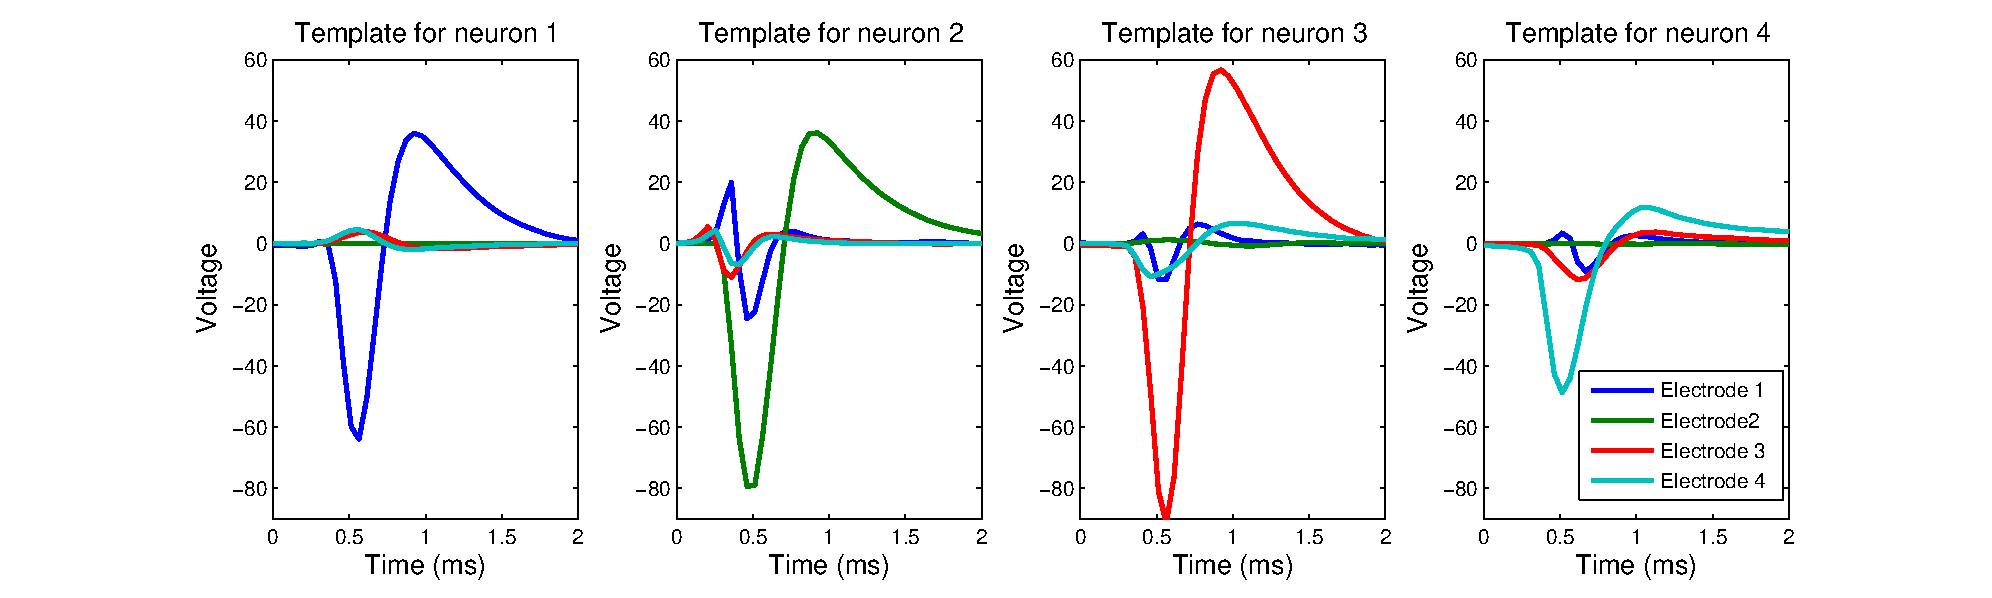
\includegraphics[width=1\textwidth]{4templates.eps} 
                \caption{Examples of action potential templates (four neurons), as recorded in four electrodes.}
\end{figure}

\subsection{The generative model}
 Denote $Y_{t,e}^{i,j}$ the observed voltage for trial $i$ of condition $j$ at time $t$ and electrode $e$. Then the model is
\begin{equation} Y_{t,e}^{i,j}=A_{t,e}^j+\sum_n^N (K_n s_n^{i,j})_{t,e}+\epsilon_{t,e}^{i,j}\quad\epsilon_{t,e}^{i,j} \sim \mathcal{N}\left(0,\sigma^2_{e,j}\right) \;\; \text{i.i.d }\end{equation}
Here $A_{t,e}^j$  is the artifact at time $t$, electrode $j$ and condition $j$, and $s_n^{i,j}$ is abinary vector containing spiking information for neuron $n$ at trial $i$ of condition $j$: $s_n^{i,j}(l)=1$ if spike occurs at time $t_{l}$. Since at most one spike per neuron occurs for a single trial, $ \sum_{l=1}^{T'}s_n^{i,j}(l)\leq1$. $K_n$ is a $(T\times E, T')$ convolution matrix whose rows contain copies of action potentials for neuron $n$ as recorded in all electrodes, but with spike onset aligned at all different possible spike times. For notational convenience, we also consider a vectorized version of equation (1), in which voltage traces are concatenated across time, electrode, trial and condition, to generate a unique huge vector $Y$. The same can be done with the artifact, spikes and neurons. This leads to the re-statement of equation (1) as
\begin{equation}
Y=XA+Ks+\epsilon
\end{equation}
Where $\epsilon \sim \mathcal{N}(0,\Sigma)$, $\Sigma$ with diagonal given by the $\sigma^2_{e,j}$'s  and $X$ is the covariate matrix that indicates which artifact variables are active in the different positions of the vector $Y$. The likelihood is thus
$$p(Y|A,s,\Sigma)\propto \exp\left(-\dfrac{1}{2}(Y-XA-Ks)^t\Sigma^{-1}(Y-XA-Ks)\right)$$
\\ The above gaussian likelihood can be further constrained: in equation (2) the artifact is way too flexible, and to avoid overfitting we impose regularity constrains that come from the (vague) knowledge of how the artifact is a function of time and condition. it is seen from experiments in absence of spiking that artifact is a smooth function of time in a given condition, and that also changes smoothly from one condition to the next. The only exception corresponds to conditions in which, due to the nature of the stimulation hardware, artifact changes abruptly and cannot be predicted from previous ones. We call these conditions breakpoints (known beforehand), and they induce a partition of the set $\{1\ldots J\}$ into $B$ subsets, denoted $b(j')$. This lead to ridge regression-like penalization terms of the form
$$\sum_t\sum_j ||A_{t+1,e}^j-A_{t,e}^j||^2,\;\;\forall e=1\ldots E\quad \sum_{j\in b(j')}\sum_t ||A_{t,e}^{j+1}-A_{t,e}^j||^2\;\; \forall j' =1\ldots B,e=1\ldots E$$
Which can ultimately be represented as products $A^tD_{k}A$ for suitable semi positive definite matrices $D_{k}$ \footnote{For numerical stability one may also include a matrix $D_{k}$ equal to the identity, which can be deemed as an overall regularization}. The amount of regularization in each of these terms is controlled by some regularization hyperparameters, denoted $\lambda_k$. Thus, our knowledge about artifact smoothness is expressed as follows
$$p(A|\lambda)\propto \exp\left(-\dfrac{1}{2} \sum_k \lambda_k A^tD_kA\right)$$
which of course corresponds to a gaussian prior.
%CORRECT THE FOLLOWING
Also, our knowledge about how spiking probability can be also stated in the model: We know, given the ordering of currents with condition, that the greater the condition the higher the spiking probability should be. This can be expressed using logistic regression priors for the (conditionally i.i.d) variables $r_n^{i,j}=\sum_{t'}s_n^{i,j}(t')$:
$p(r_n^{i,j}=1|\alpha_n)=\dfrac{1}{1+\exp\left(-\alpha^0_n-j\alpha^1_n  \right)}$. Regarding spike times, we set a uniform prior on the times $t_{l}$. Finally, for the variances $\sigma^2_{e,j}$ the non-informative prior $p(\sigma^2_{e,j})\propto \frac{1}{\sigma^2_{e,j}}$ is assumed, and they are also assumed independent, giving rise to a certain prior for $\Sigma$. With this generative model the goal is to jointly infer $s$ and $A$.
\subsection{Relation to other methods}
\section{The Algorithm}
With the above generative model, the first impulse is to follow the MAP approach: what are the most likely spike allocations and artifact that allow us to explain the data, given our prior knowledge? There are, though, several caveats: First, the introduction of the binary vector $s$ renders the problem non convex, which implies many local optima may exist. Thus, we are at risk of obtaining meaningless local solutions. Also, there are regularization hyperparameters that need to be estimated somehow. Third, all models are wrong and, as a consequence, there is not guarantee that MAP solution will provide the right spike sorting. To address these issues, and improve robustness to model misspecification and initial values, the inference procedure is divided into four stages steps, which, put together, give rise to the spike sorting algorithm

\subsection{Data cleaning}
The first step is to throw away non useful data: We only consider voltage traces until a time there are chances to observe a spike, possible followed by a short time window to correctly capture the effects of action potential of late spikes. Also, not all the electrodes are considered: experience shows that considering too many electrodes may worsen performance, as if in some of then the action potential signals is not strong enough, one may end up trying to fit noise. Also, addition of electrodes may create computational bottlenecks in some parts of the algorithm. The rule of thumb is: choose as many electrodes as neurons are being analyzed, obviously with that electrode being the one with the strongest signal for each neuron (if that electrode is shared by different neurons, choose the second with strongest signal).

 \subsection{Initialization}
 As mentioned before, multimodality implies that any optimization (or sampling) procedure is prone to fall into local optima, and this local optima may be non interesting. It is of critical importance to come up with good initial estimates of the parameters in order to avoid such situations. To this end, we consider initial values provided by a convex relaxation, explained below.
 
 \subsubsection{Convex relaxation via SOCP}
 
We turn the original estimation problem into a convex one by allowing the binary vectors $s_n^{i,j}$ belong to the $T'-$simplex: $0\leq r_n^{i,j}\equiv \sum_{l=1}^{T'} s_n^{i,j}(l)\leq 1, 0\leq s_n^{i,j}(l)\leq 1$. In this new setting we no longer look for spikes but rather 'generalized spikes', and the presence or absence of spikes at certain times is replaced by spike probabilities. Unfortunately, even if the new problem is already convex, there are some nonlinear dependencies (for example, with the logistic regression, artifact regularization and variance priors) that impose hard computational constraints for the maximization of the log posterior. Thus, our approach is to re-state an approximation of our already convexified problem in a framework for which a number of efficient solvers are available. To this end we profit from the Second Order Cone Programing (SOCP) theory, in which a linear function is minimized, subjected to conic constraints. The question is how to come up with an approximation that captures the spirit of the original program. We take the following approach: to avoid artifact regularization hyperparameters, we consider instead a simple polynomial model; artifact is unconstrained in time but assumed a polynomial function of condition (with conditions in the same set $b(j')$). This leads to the replacement of artifact  $XA$ by a product $X'A'$, with $A'$ the new artifact variables and $X'$ representing covariates in this polynomial representation. The logistic regression prior is replaced by the (linear) constraint that spiking probabilities increase with condition, for each neuron. That is, for $j=1\ldots J-1$ and $n=1\ldots N$ we set $\sum_{i,l}s_n^{i,j}(l) \leq \sum_{i,l}s_n^{i,j+1}(l)$. Finally, the non-informative prior for the variances is just avoided.\\
Before stating the SOCP in detail, notice that artifact and spike variables can be concatenated, by defining $z=(A',s)$. In the same vein, the artifact plus (generalized) action potential term can be expressed as a unique matrix product between some matrix $M$ and $z$. \\
Now, let's construct the new program: first, to make the relaxation as similar to the original program as similar as possible, we will look for sparseness in the generalized spiking vectors. This translates in imposing not only simplex constraints but also in penalizing spiking in the objective function via the linear term $\sum_{j,i,n,l} s_n^{i,j}(l)$. Notice this will naturally induce sparseness, as $s_n^{i,j}(l)=|s_n^{i,j}(l)|_1$.  With this, we now need to state we want to explain our data (log likelihood). We do so by a quadratic term for each condition: we want the RSS $||Y-Mz||^2$ to be as small as possible. To meet the linear objective requirement for a SOCP,  we use duality and introduce the auxiliary variable $\rho$ in the objective and constraint $||Y-Mz||^2\leq \rho$. The trade-off between explaining of the data and sparseness is modulated by the hyper parameter $\kappa$, which is set beforehand. \\Summarizing, we aim to solve the following problem
  \begin{eqnarray}& \displaystyle{\min_{z=(A',s),\rho}\quad \quad  \sum_{j,i,n,l} s_n^{i,j}(l)+\kappa \rho} \\ \nonumber
  \text{s.t. } & 0\leq\sum_{l=1}^{T'} s_n^{i,j}(l)\leq 1\;\;\forall i,j,n\quad 0\leq s_n^{i,j}(l)\leq 1\;\; \forall i,j,n,l \quad \text{generalized spikes}\\ \nonumber
  & \sum_{i,l}s_n^{i,j}(l) \leq \sum_{i,l}s_n^{i,j+1}(l)\quad \forall n, j=1\ldots J-1 \quad \text{increasing spiking probabilities}\\ \nonumber 
  & ||Y-Mz||^2\leq \rho \quad \quad \text{ Explaining data} \\ \nonumber
\end{eqnarray}
 
There are two concerns with this formulation: First, different choices of the new parameters ( $\kappa$, and the degree of the polynomial) will lead to different initial solutions. However, results show that it is a good choice to set high values of $\kappa$, which represents the importance of explaining the data over sparseness of the generalized spikes. For the degree of the polynomial, satisfactory results are achieved with a quadratic model. There is no need to increase this degree further as this would lead to more variables, and as a result, slower computations. Also, as mentioned above, we are solving an approximation,  and for example, the obtained spike probability v.s. condition curves (thereon spike activation curves) may look non-smooth. However, again results show the approximated results provided by this SOCP are good enough to provide initial estimates for the variables of the problem. Now we give details about how to obtain initial values of the variables given the solution of the SOCP. \\
\subsubsection{Initialilzation of $A,\Sigma, \alpha$ and $\lambda$}
Obviously, initial value for the artifact will be given by $A_0=XA'$, where $A'$ is the solution of the SOCP. Also, for $\Sigma_0$ we look for the residuals at different conditions and electrodes, leading to
$\sigma^2_{{j,e}_0}=\frac{1}{TI}||Y_{j,e}-M_{j,e}z||^2$ where $Y_{j,e}$ and denotes the sub-vector of $Y$ obtained by considering only samples in condition $j$ and electrode $e$, and $M_{j,e}$ is the sub matrix of $M$ constructed in a similar manner. \footnote{Notice the above estimates are biased and should be corrected by the number of degrees of freedom, however, this has little impact in results and thus this further step is avoided.}
\\For $\alpha$, the parameters of the logistic regressions, we consider a least square fit with the activation curves. Finally, for $\lambda$, we carry out maximization of $p(A_0|\lambda)$ with respect to $\lambda$. This leads to the following problem
\begin{eqnarray}\nonumber & \lambda_0=\arg\min_\lambda \frac{1}{2}A_0^t\left(\sum_{k}\lambda_k D_{k} \right)A_0-\log \bigg|\sum_{k}\lambda_k D_{k}\bigg|\\ \nonumber & \text{s.t.} \quad  \lambda\geq 0\\ \nonumber & \sum_{k}\lambda_k D_{k} \succ 0
\end{eqnarray}
The above (convex) problem is known in the literature as \textit{maxdet}, and to solve it we use gradient descent.
Notice the only parameter we have not initialized is the first estimate of the spikes $s_0$. However, this is not necessary, as this will arise as a consequence of the next step of the algorithm: Gibbs sampling. For now, it is enough to have initial estimates of the generalized spikes, which were given by the SOCP. 
\subsection{Gibbs sampling}
Given our initial solution we would like to converge to obtain good local optima of the posterior. That can be done via coordinate descent between $A,s,\Sigma,\alpha$ and $\lambda$. However, to keep the probabilistic set up in mind, and to allow more variability in solutions (and a better exploration of the parameter space) we prefer a block Gibbs sampling approach. Notice that in any case solutions shouldn't be very different (and they are not in practice), as the posterior is highly peaked in the modes, given the overwhelming weight of the likelihood. Thus, coordinate descent becomes essentially equivalent to Gibbs sampling, where the samples will correspond (approximately) to the modes.
\\Now we detail the several stages of the Gibbs sampler
\subsubsection{Sampling from spikes}
The conditional spike probabilities for a neuron at a given trial and condition, given all the rest of the variables and data is multinomial:
$$p(s_n^{i,j}(l)=1|Y,A,\Sigma,\lambda,\alpha,s\backslash_{n}^{i,j})\propto \frac{p(r_n^{i,j}(l)=1|\alpha_n)}{T'}\exp\left(-\frac{1}{2}\sum_e \frac{||Y_e^{i,j}-\sum_n (K_n  s_n^{i,j})_e-A^j_e||^2}{\sigma^2_{e,j}}\right)$$
Notice posterior spike probabilities of a given trial don't depend on other trials or conditions. However, spiking in one neuron does depend on spiking from others. This leads to a sequential sampler: we iteratively sample from different neurons while keeping spikes of the others fixed, and within each neuron, we sample all trials and conditions.
\subsubsection{Sampling from the artifact}
Denoting $\Lambda=\left(\sum_k \lambda_k D_k\right)^{-1}$ we have the following expression for the conditional distribution of the artifact, conditional on the rest of the variables and data.
$$A|Y,s,\Lambda,\Sigma,s,\alpha\sim \mathcal{N}(\mu,\Sigma')\quad \Sigma'=\left(X^t\Sigma^{-1}X+\Lambda^{-1}\right)^{-1}\quad \mu=\Sigma'X^t\Sigma^{-1}(Y-Ks),$$
\subsubsection{Sampling from $\Sigma$}
Sampling is straightforward once noticing that the conditional distribution of $\sigma^2_{e,j}$ conditional on data and the rest of variables is inverse gamma:
$$\sigma^2_{e,j}|Y,s,A,\alpha,\lambda,\sigma^2\backslash_{e,j}\sim\text{ Inv-Gamma}\left(\frac{ITE-1}{2},\frac{1}{2}||(Y-AX-Ks)^j_e||^2\right)$$
\subsubsection{MAP for $\alpha$}
Notice we implicitly assume a flat prior for $\alpha$. One may sample from it's posterior distribution, but in order to keep simplicity we prefer a maximization approach \footnote{Notice by doing thus we no longer have a \textit{bona fide} Gibbs sampler, but instead, a Gibbs-EM hybrid}:
$$\max_{\alpha} p(\alpha|s,A,Y,\Sigma,\lambda)\propto \prod_{i,j,n}\frac{1}{1+exp\left(-(2r_n^{i,j}-1)(\alpha_n^0+j\alpha_n^1)\right)}$$
The above maximization corresponds is achieved by performing $N$ separate logistic regressions, one per each neuron.
\\
Regarding $\lambda$, we don't further modify from this variable from its inicial value. There are two reasons for not doing so: first, we may end up in artifact overfitting, so it is preferable to have a value of this hyper parameter as a 'point of truth'. We have already obtained an estimate for this value, $\lambda_0$, and results show this choice is already good enough. Also, optimizing  $\lambda$ via solving the maxdet problem at each iteration would create a huge computational bottleneck. \\
Via repeated iterations of the several stages of the Gibbs sampler, convergence to points close to local optima is achieved. Hopefully this solution corresponds to the right spike sorting, and this is the case sometimes, but in general one may obtain nonsensical spike trains: the most typical situations corresponds where the spike sorting is correct for some conditions, but there are others in which no spikes are found, where in reality all trials have spikes, or vice versa. Also, it is possible to infer spike in all trials while spikes are present only in some of them. Fortunately, there are ways to diagnose this pathological, though common, situations, and these diagnostics allow us to come up with the last part of the algorithm, which is a post-processing heuristic that introduces local changes in the Gibbs sampling solution, in order to improve the fit in the aspects where an overt lack of sense has been diagnosed.
\subsection{Post processing}
There are two ways to assess the plausibility of solutions provided by Gibbs sampling: the first of them is to look at the RSS at each condition. In conditions where the fit is poor these residuals should be higher. The problem of just looking at the residuals is that there are other reasons that could make the RSS to be high: the response of the neural system changes from one condition to the next, and there are phenomena characteristic to each condition but not  accounted for by the model that explain significant conditions\\ A more amenable alternative comes from assessing differences between empirical spiking probabilities at each condition, $\sum_i r_n^{i,j}/I$, and probabilities of spiking provided by the logistic regression, $\hat{p}(r_n^{i,j}=1)$. As we are confident that logistic regression is a good description os reality, lack of fit in this aspect of the model diagnoses the attained solution doesn't explain data in the desired sense. In those cases, something is needed to be done to 'jump' from this local optima into a better one. This is done by re-sampling the artifact in the conditions where the fit is worst conditional on the rest of the  sampling from the conditional (prior) distribution of the artifact given the rest of the conditions. That is, if $J_1$ is the set of such conditions, we re-sample the artifact from $p(A_{J_1}|\lambda,A\backslash_{J_1})$. Sampling is straightforward because of the gaussianity of the above conditional distribution. In other words, we 'borrow' statistical strength from places where we are confident the fit is good. The above idea can be implemented as an heuristic: briefly, re-sample the artifact and with this new estimate re-sample spikes and the rest of variables. Assess the fit again, until we cannot reject the hypothesis that spikes come from a logistic regression model (using a chi squared test, see \cite{Hosmer1997}) , or until a maximum number of iterations is exceeded. Notice this is similar to the use of the minimum discrepancy $D_{\min}$ \cite{Gelman96posteriorpredictive} in a posterior checking framework, but unfortunately we were not able to explore other bayesian criticism measures \cite{Box1980}, because of the difficulty of sampling from this highly peaked and multimodal posterior distribution. 
\\Before comenting results, in figure 2 are shown all the stages of the algorithm in a sample dataset.
\pagebreak 
   \begin{figure}[ht!]
        \centering
        \begin{subfigure}[b]{0.5\textwidth}
                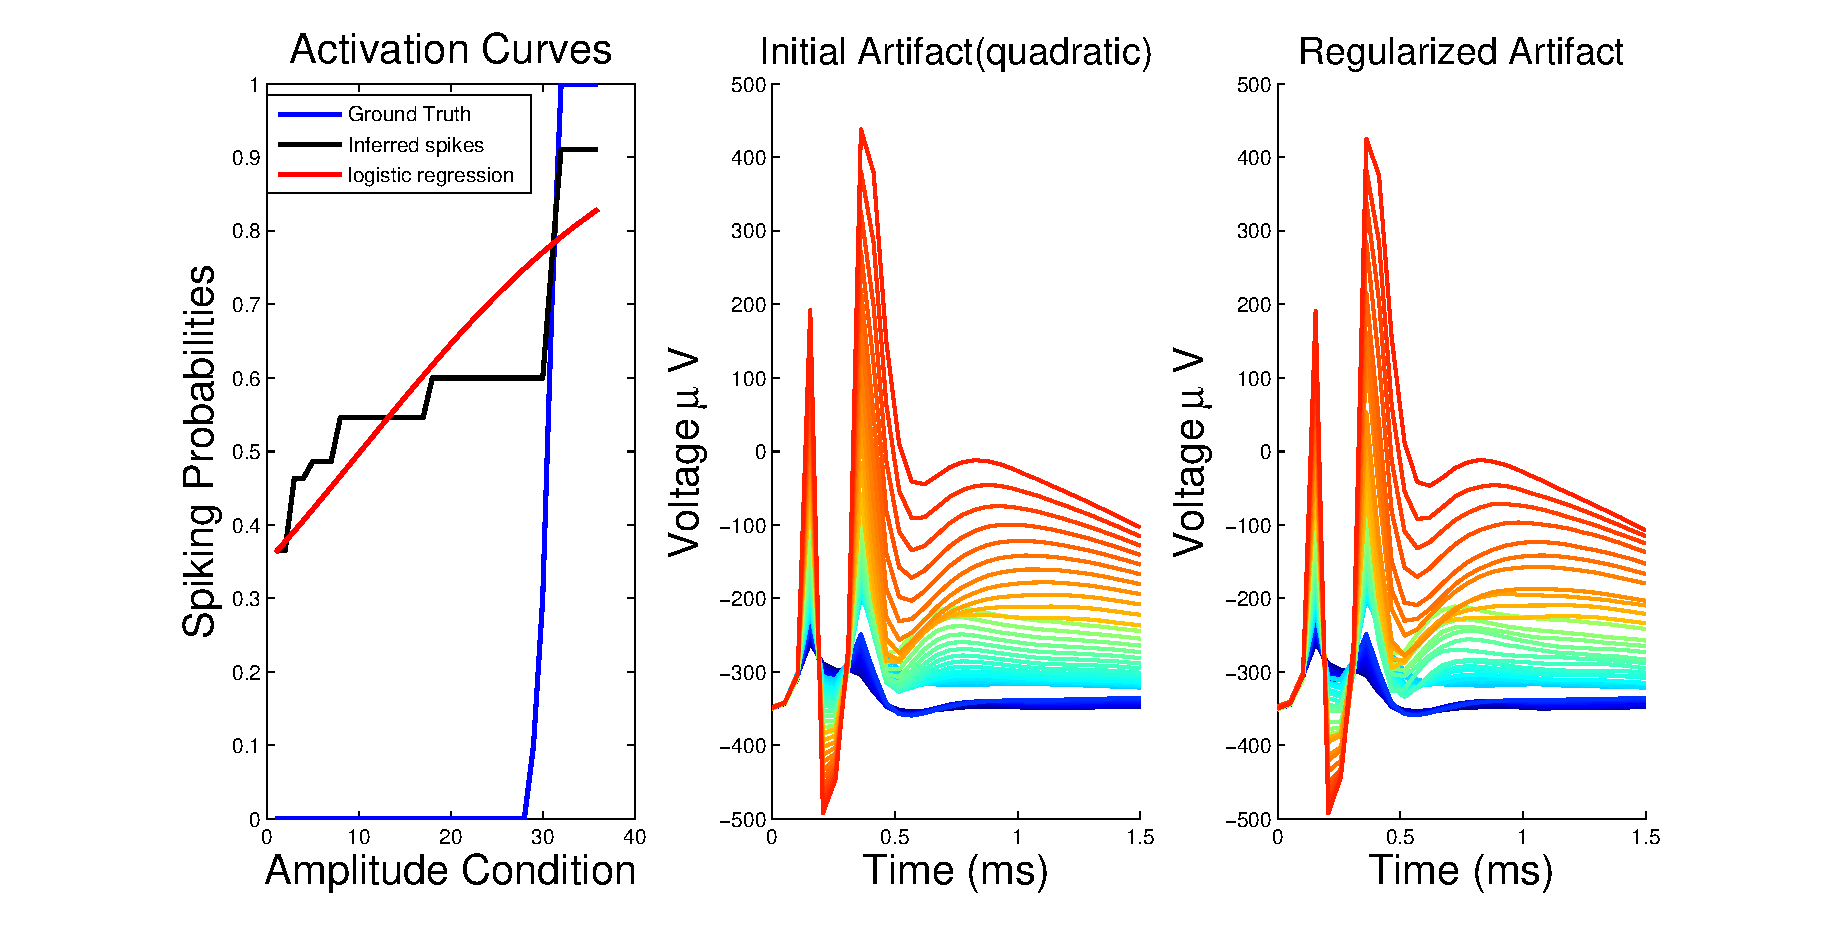
\includegraphics[width=\textwidth]{i0.eps}
                \caption{After Convex relaxation}
                \label{fig:gull}
        \end{subfigure}% 
~\begin{subfigure}[b]{0.5\textwidth}
                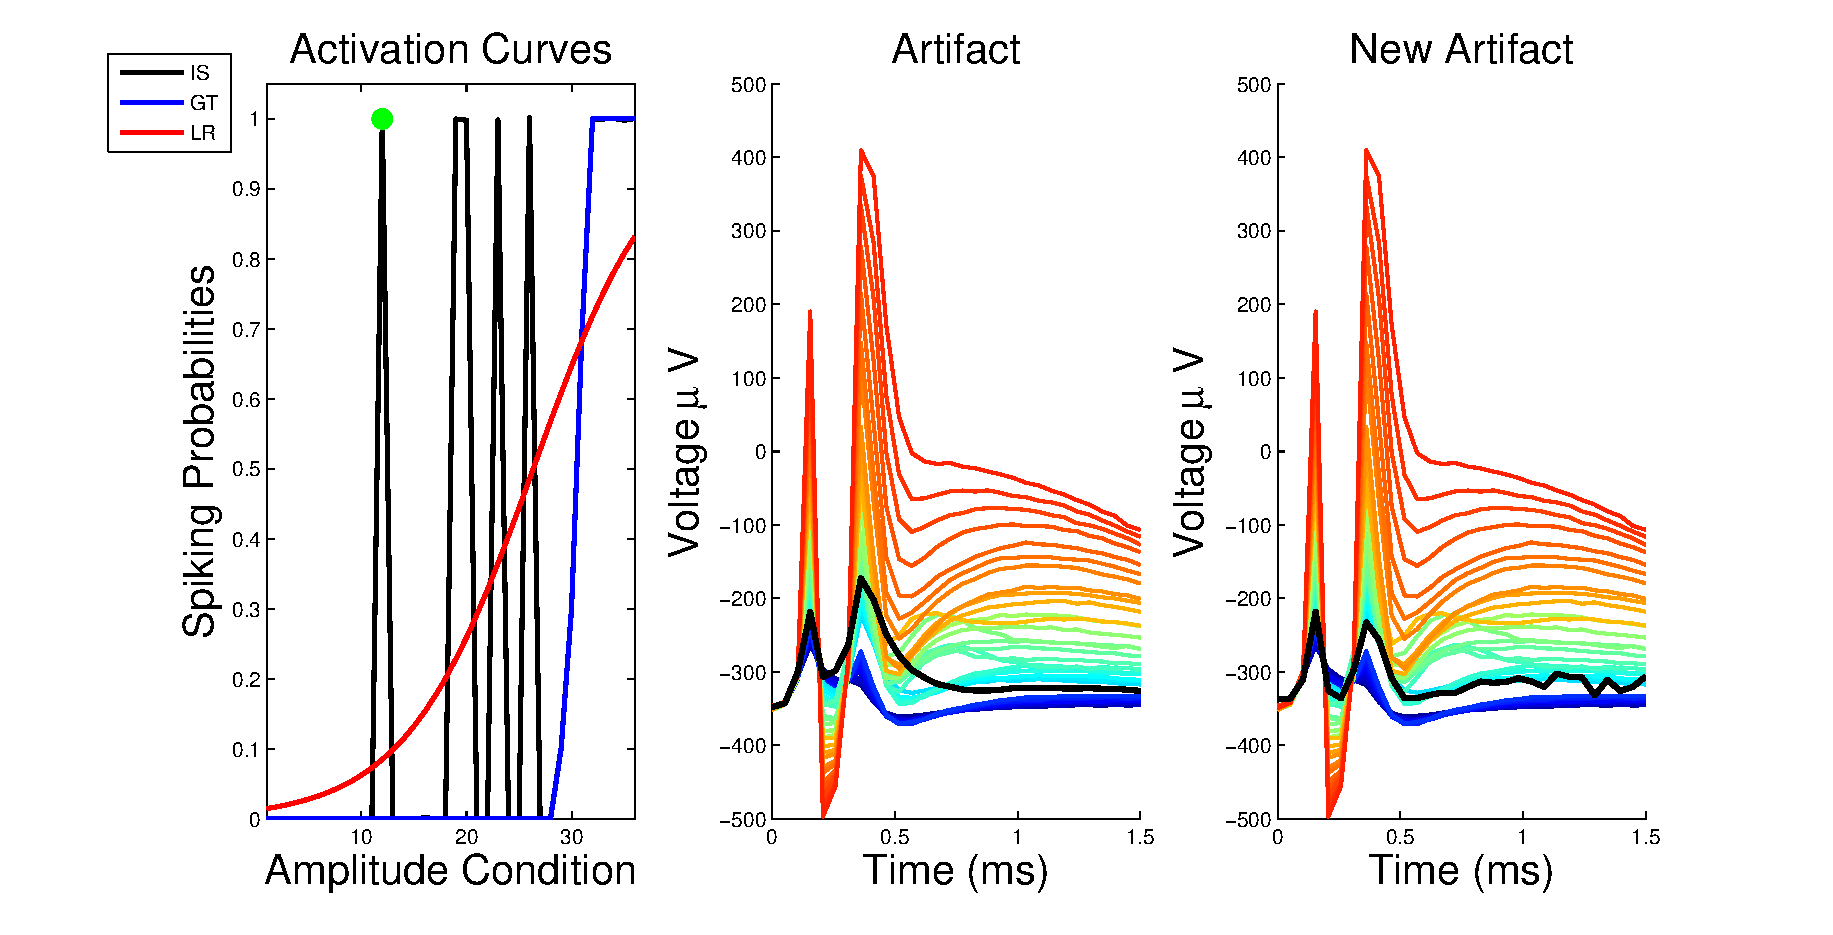
\includegraphics[width=\textwidth]{i1.eps}
                \caption{Gibbs Sampler Solution}
                \label{fig:tiger}
        \end{subfigure}
 
        \begin{subfigure}[b]{0.5\textwidth}
                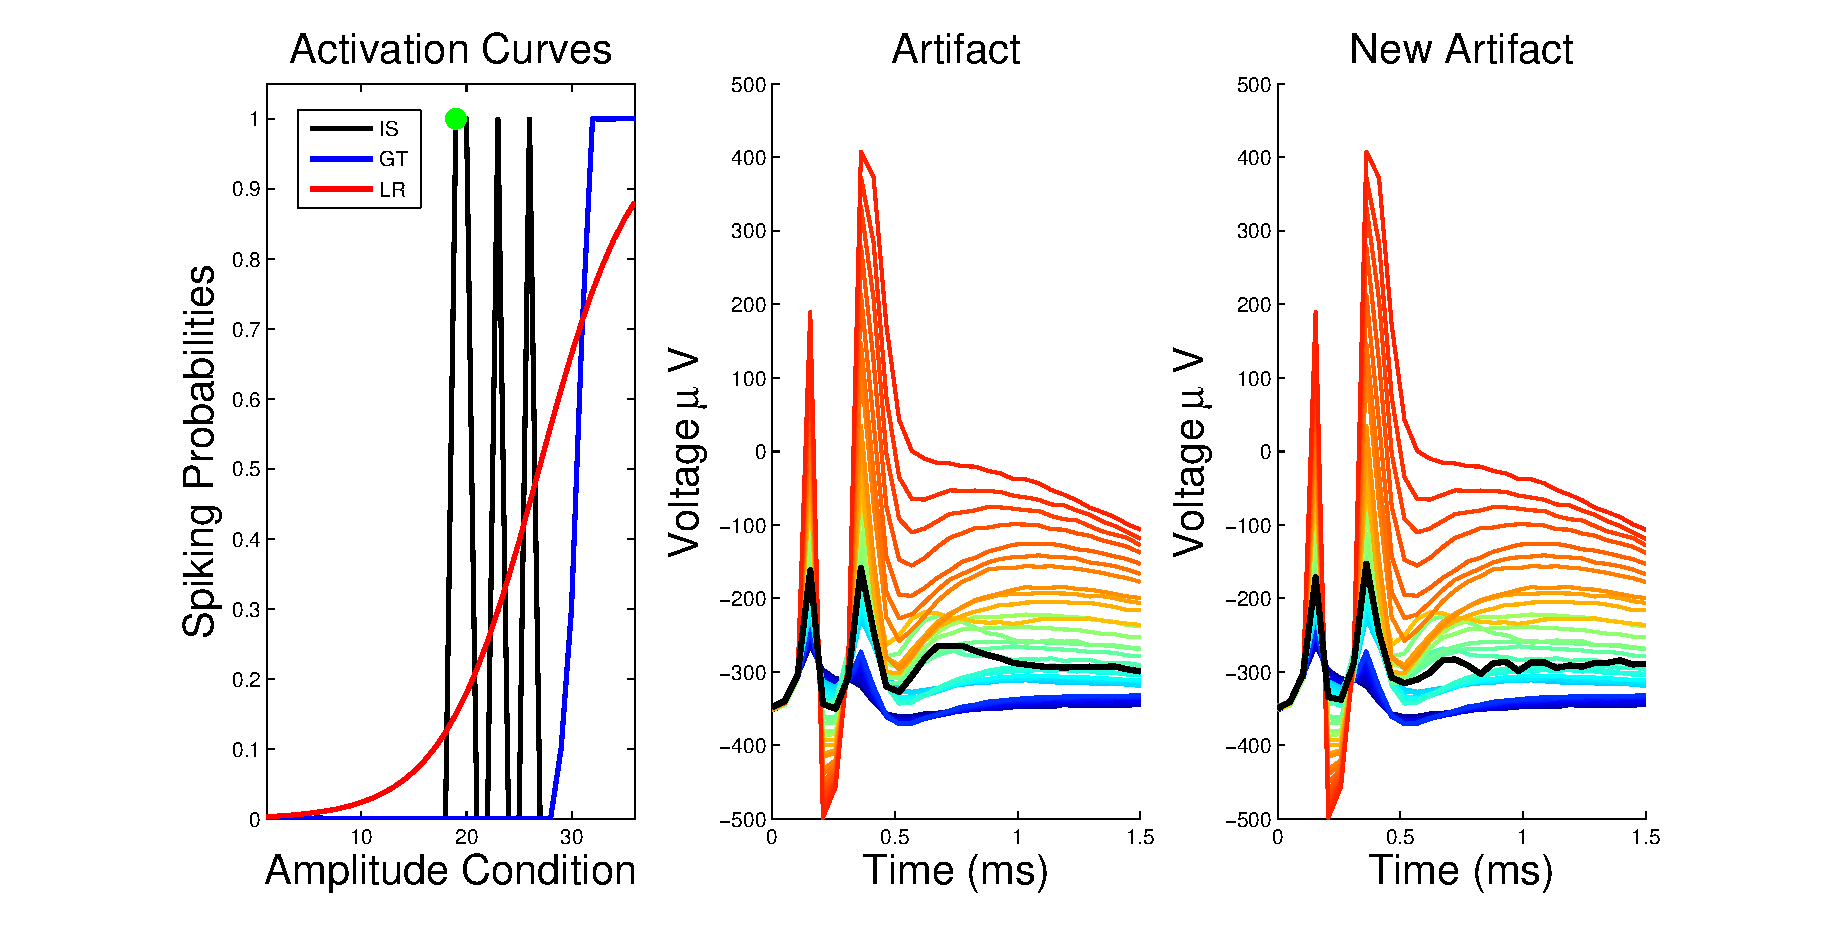
\includegraphics[width=\textwidth]{i2.eps}
                \caption{After one iteration of heuristic}
        \end{subfigure}~
         \begin{subfigure}[b]{0.5\textwidth}
                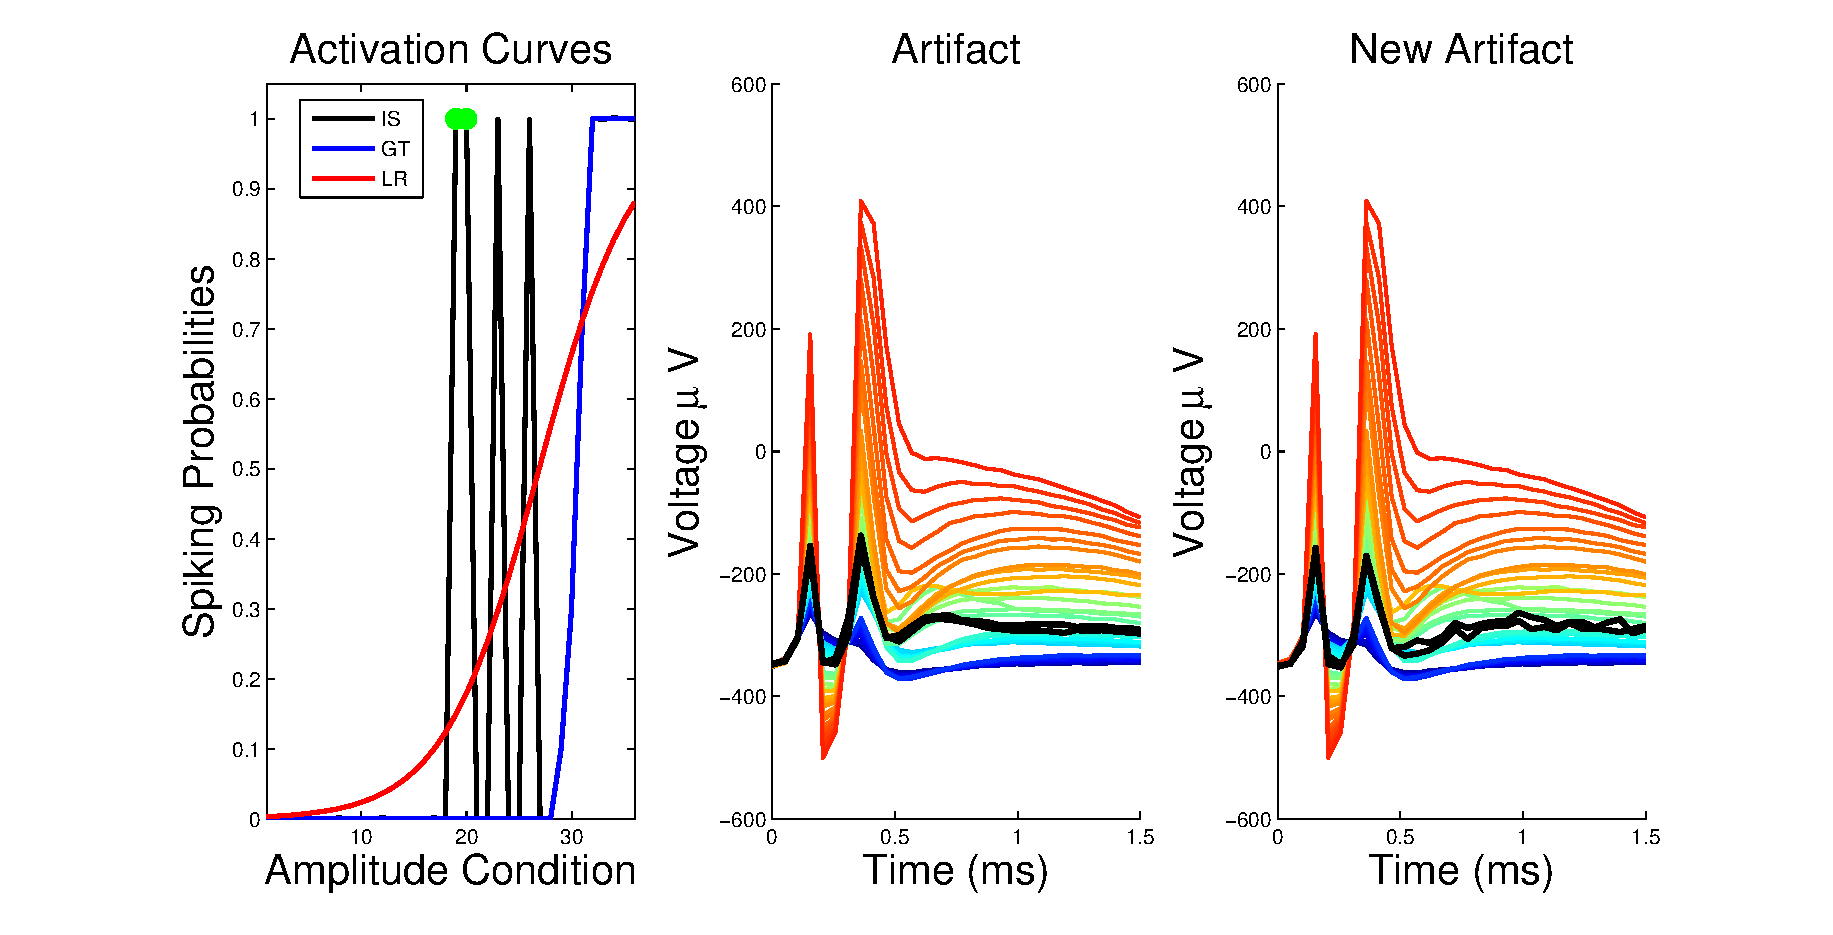
\includegraphics[width=\textwidth]{i3.eps}
                \caption{After two Iterations of heuristic}
                \label{fig:mouse}
        \end{subfigure}
        
        
        \begin{subfigure}[b]{0.5\textwidth}
                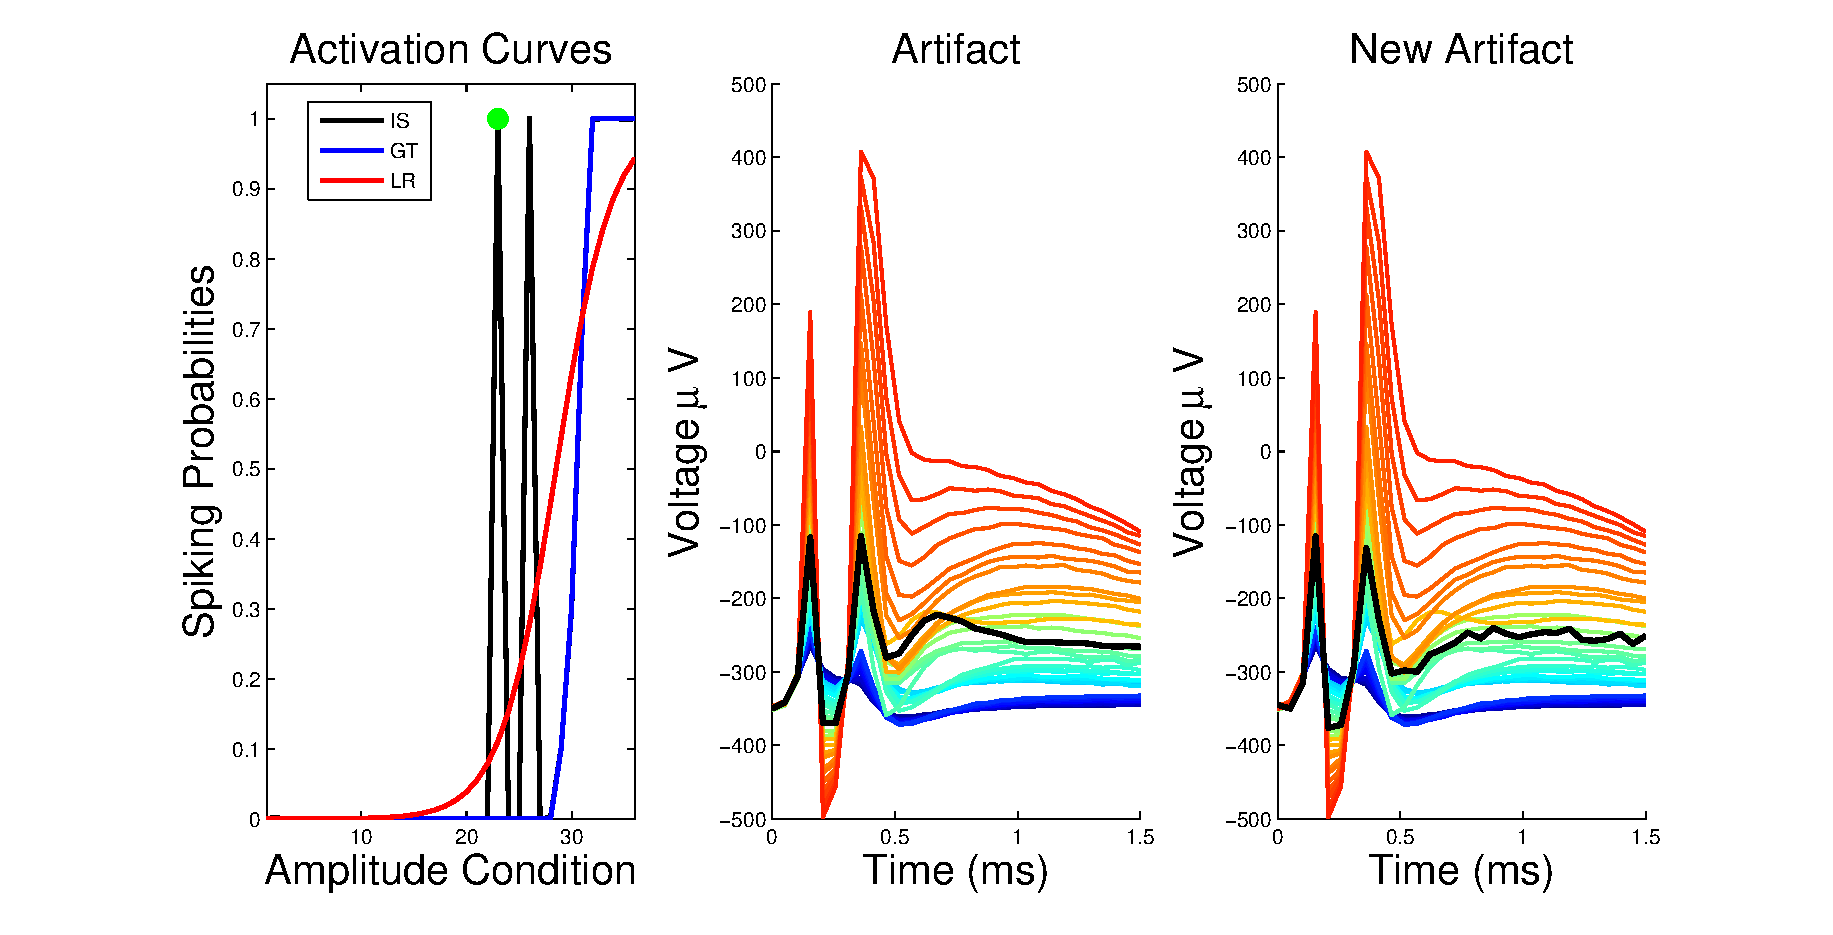
\includegraphics[width=\textwidth]{i4.eps}
                \caption{After three Iterations of heuristic}
        \end{subfigure}~
         \begin{subfigure}[b]{0.5\textwidth}
                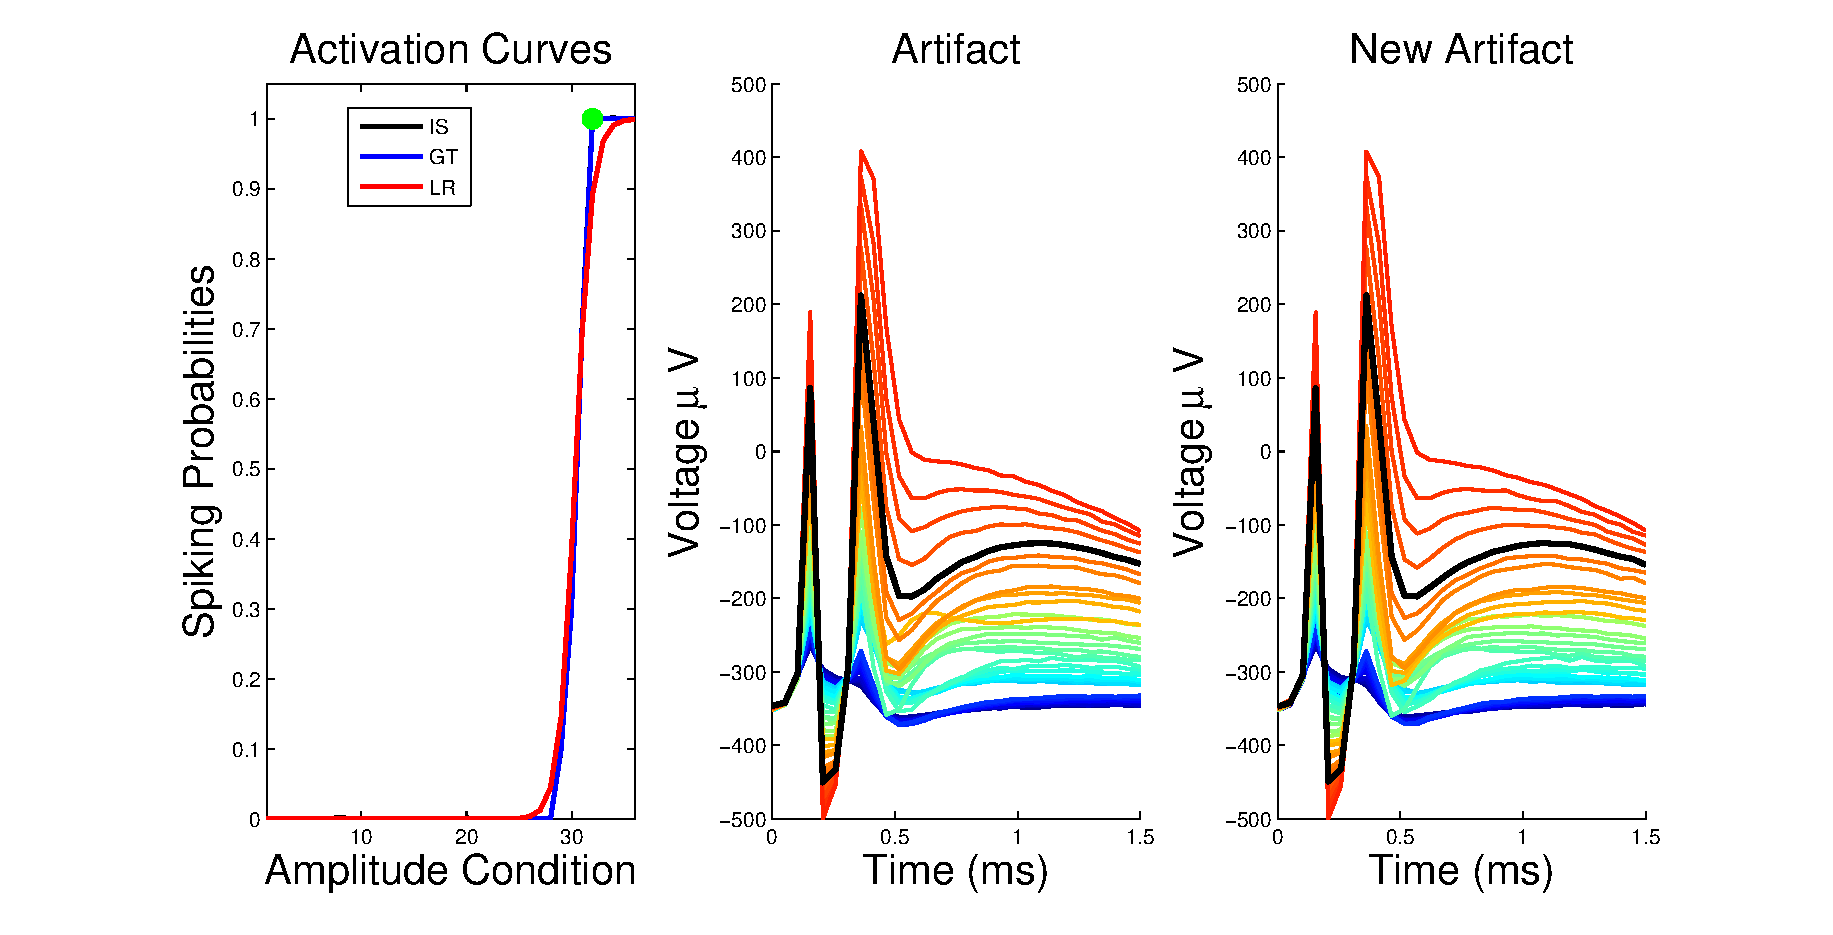
\includegraphics[width=\textwidth]{i6.eps}
                \caption{Final Result}
                \label{fig:mouse}
        \end{subfigure}
\caption{Illustration of the different stages of the algorithm. Initial values provided by the convex relaxation (a) are used as input for the Gibbs sampler (b). If the fit of the activation curve to a logistic model is poor, the artifact is resampled in the conditions that are most responsible of that lack of fit (c,d,e), until no changes are further needed (f)}
\end{figure}


    \section{Results}
    The algorithm was tested in 56 datasets in which spike sorting was required for 4 neurons (templates in the electrodes used are shown in figure 1). For all of them the number of amplitude conditions was 17, and for each condition there were either 20 or 10 trials. In the former performance was almost perfect, with an overall error rate of 0.71\% (see table 1 for summary results for each neuron and figure 3 for the true and estimated activation curves). However, in the latter the error rate was higher, reaching 10.9\% (see table 2 for details), possibly due to the limitations posited by the fewer number of trials. As we aim to decrease the error rate to zero, it is important to understand better which are the causes of failures: Better models can be built if these causes are well understood, and even with the current model this understanding could be used to inform the human expert when the causes are present. It turns out that the unwanted activation of an axonal bundle is the phenomenon that explains the best failures in spike sorting. In the following we show how this axonal activation hampers spike sorting, and how to deal with it in the absence of a better model
    \begin{table}[h!]
\begin{tabular}{|c|c|c|c|c|c|}
\hline
   &  Trials w. spikes & Failures in detection & Trials w. no spikes & False positives  & Total \\ \hline
   Neuron 1 & 1040 & 43 ( 4.1 \%)& 2190 & 73 (3.3\%) & 3230 \\ \hline
   Neuron 2 & 329 & 0 & 2901 & 1 (0.03\%)  & 3230 \\ \hline
   Neuron 3 & 546 & 0 & 2684 & 0 & 3230  \\ \hline
   Neuron 4 & 310 & 0 (.64\%) & 2920 & 39 (1.33\%) & 3230  \\
  \hline
\end{tabular}
\caption{Overall results for all the analyzed neurons (only 10 datasets with 20 trials per condition)}
\end{table}
\begin{figure}[h!]
          \centering
                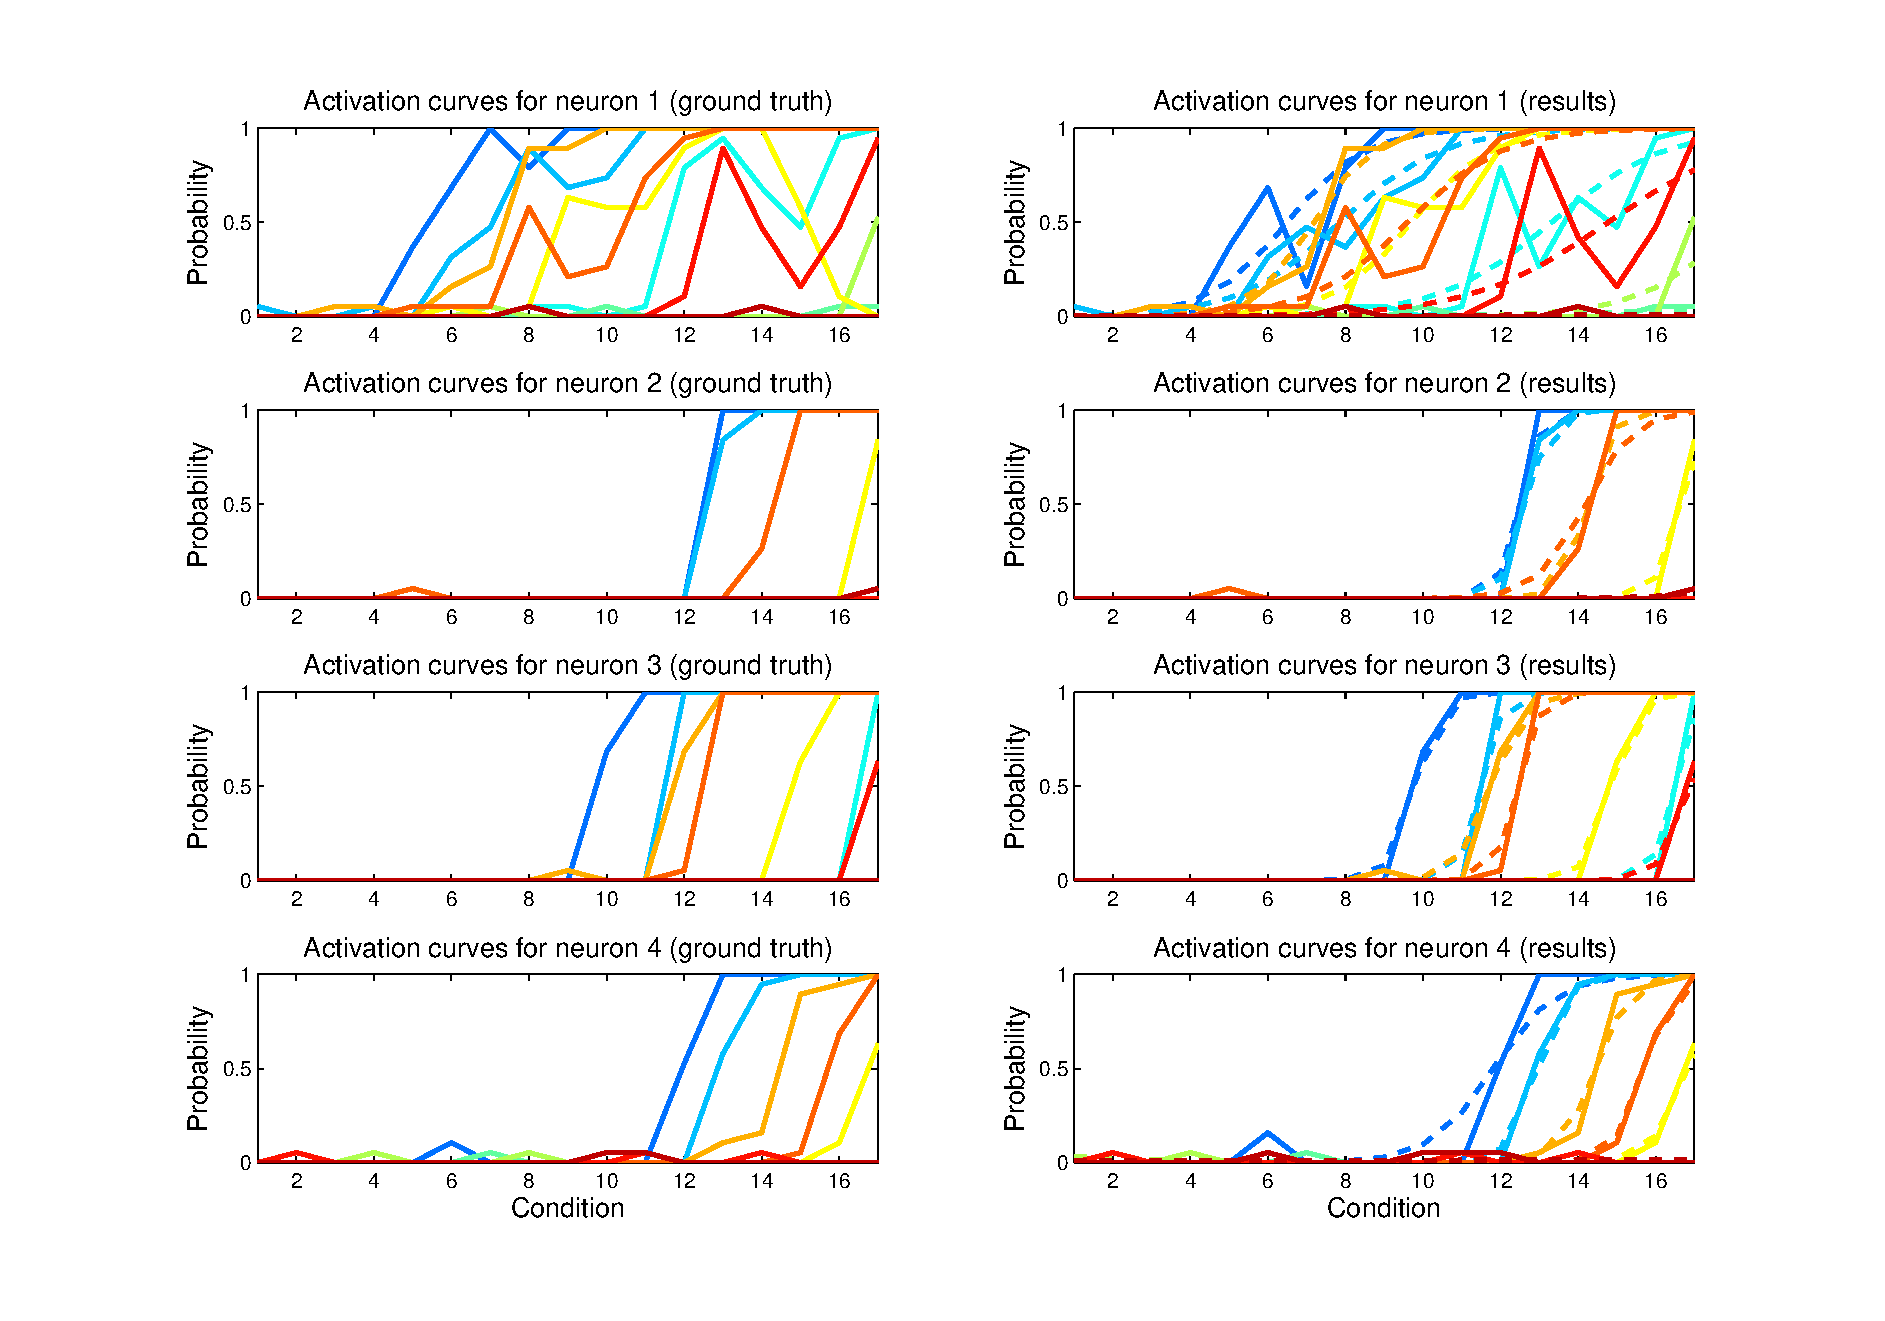
\includegraphics[width=1\textwidth]{Results10datasets.eps} 
                \caption{Activation curves, ground truth (left) and model results (right). Each trace corresponds to a dataset. In the  plots  to the right are also shown (dashed lines) the logistic regression fits}\end{figure}

\begin{table}[h!]
\begin{tabular}{|c|c|c|c|c|c|}
\hline
   &  Trials w. spikes & Failures in detection & Trials w. no spikes & False positives  & Total \\ \hline
   Neuron 1 & 4328 & 1019 (23.5\%) & 5940 & 490 (8.26\%) & 10268 \\ \hline
   Neuron 2 & 3515 & 689 (19.56\%) & 6236 & 519 (7.68\%)  & 10268\\ \hline
   Neuron 3 & 1498 & 0 & 8488 & 282 (3.22\%)& 10268  \\ \hline
   Neuron 4 & 2143 & 124 (5.79\%) & 7159 & 491 (11.89\%) & 10268  \\
  \hline
\end{tabular}
\caption{Overall results for all the analyzed neurons (all the 56 datasets)}
\end{table}


        \subsection{Misspecification due to axonal activation}
 It has been recently documented \cite{Lauren2014} that besides action potentials elicited by the targeted electrical stimulation of somas, there can be unwanted activation of axons. This activity can also be detected in electrode recordings, and although it is still not completely understood, it is known that begins to appear at a similar amplitude that of somatic spikes. However, unlike somatic spikes, the magnitude of this aggregated activation of axons increases with stimulus amplitude, and the activation curves of these axonal activities tend to be much sharper than of spikes. Because of this, templates are not available for this bundle activation and as a result it cannot be easily accounted for in the current framework. 
 \\ Axonal activation thus leads to model misspecification, and the question is to which extent our misspecified model can still be useful to detect spikes, in other words, will this phenomenon affect algorithm performance, and if it does, is it possible to inform a possible failure, in order to proceed with manual detection?\\
To address this questions we proceed via examples. In figure 4 is shown an example of successful detection (although it doesn't coincide with ground truth) regardless of the presence of axonal activation. This example serves to illustrate a way in which axonal activation interacts with the rest of the components of the model: here, spikes have a bigger magnitude than the corresponding template, and this is explained by the overlap in time of somatic and axonal spikes. Thus, we detect onset of axonal activation by increased residual variance $\sigma$ (in this case conditions 11 or 12). Also, once axonal activation becomes less variable in time, it is treated by the algorithm as being part of the artifact, which explains the difference in red and black traces at conditions 14 and 15. There are some cases, however, where the spike shapes change so much due to axonal activation that the templates are not good enough to explain the residuals and as a result spikes are failed to be detected. This is a rare situation, and again, it should be identified by an increased residual variance. An example of failure is shown in figure 5. There are conditions (e.g. 6,7) in which clusters naturally into three classes: no spiking, spiking and spiking plus axonal activation. At conditions 7 and 8 spikes are not detected, and only spike plus axonal activation trials are considered as true spikes (in fact, the same judgement was made by the human at condition 8). To understand how things can go wrong here it is important to look at the residuals: In some sense, it is also a meaningful interpretation to believe blue traces in condition 7 have no spikes, because if that was the case the spike template would fairly match the residuals. This example shows how spike sorting requires a level of expertise that is beyond what can be stated in the model. However, again in this case presence of axonal activation is indicated by increased residual variance, which can be informative for the experimenter. Other examples (not shown here) include similar situations, and an erroneous spike detection could be detected by a lack of fit between the activation curves and the underlying logistic model. Finally, another measure that can be informative comes from the regularization prior: basically, one can ask the question of how plausible is our artifact estimate given our prior artifact specification. If not, that could indicate that a artificial breakpoint should be added to the model in order to properly account for the changes in the artifact induced by the axonal activation. 
\\Summarizing, this modeling framework is not exempt of risks due to misspecification, but we can evaluate the goodness of fits by looking at different relevant aspects of the model: underlying spike probabilities, residual variances, and prior artifact specification. Taken together they should lead to relevant information about possible lack of fit, causes of this lack of fit (axonal activation) and ways in which this lack of fit could be driving the results wrong.
\pagebreak
\begin{figure}[h!]
          \centering
                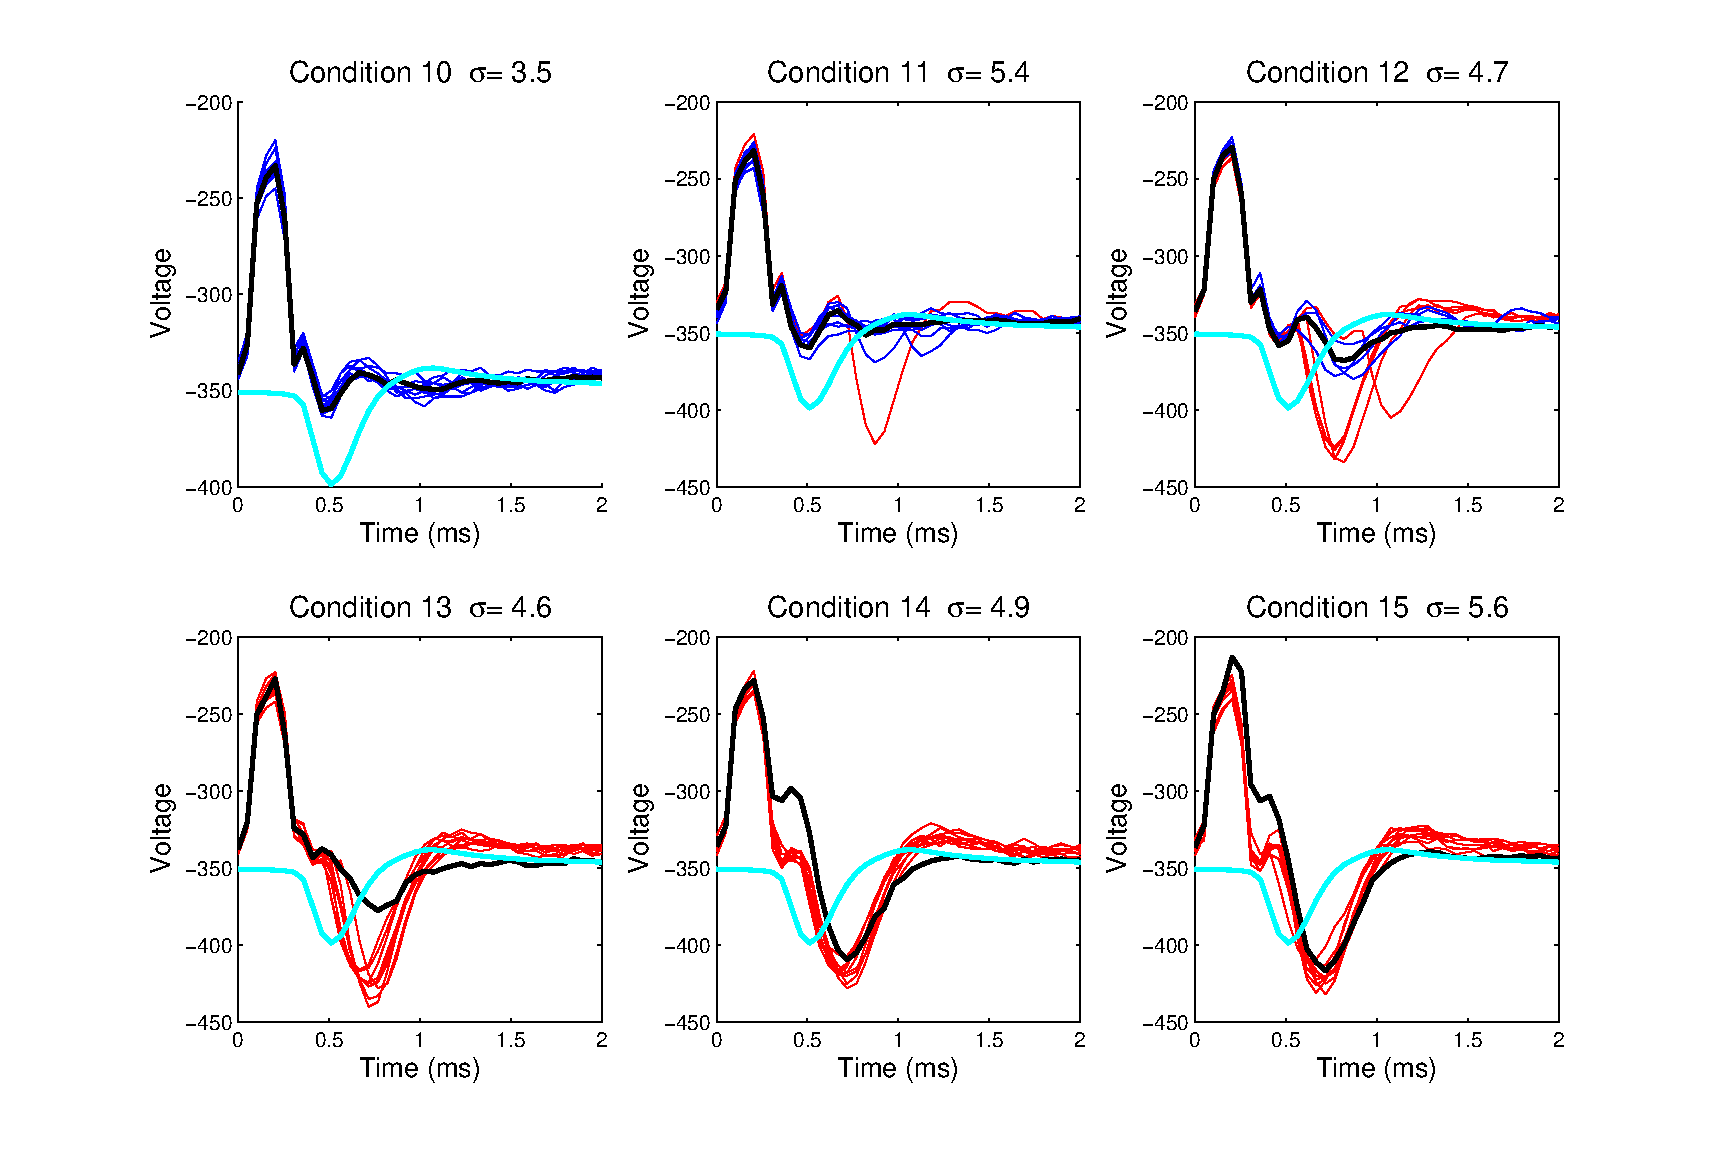
\includegraphics[height=4in]{TracesEl185pattern1494.eps} 
                \caption{An example of successful detection with axonal activation. Cyan trace: spike template, blue traces: trials with no spike, red traces: trials with spikes, black: artifact estimate}
\end{figure}


 \begin{figure}[h!]
        \centering
        \begin{subfigure}[b]{\textwidth}
                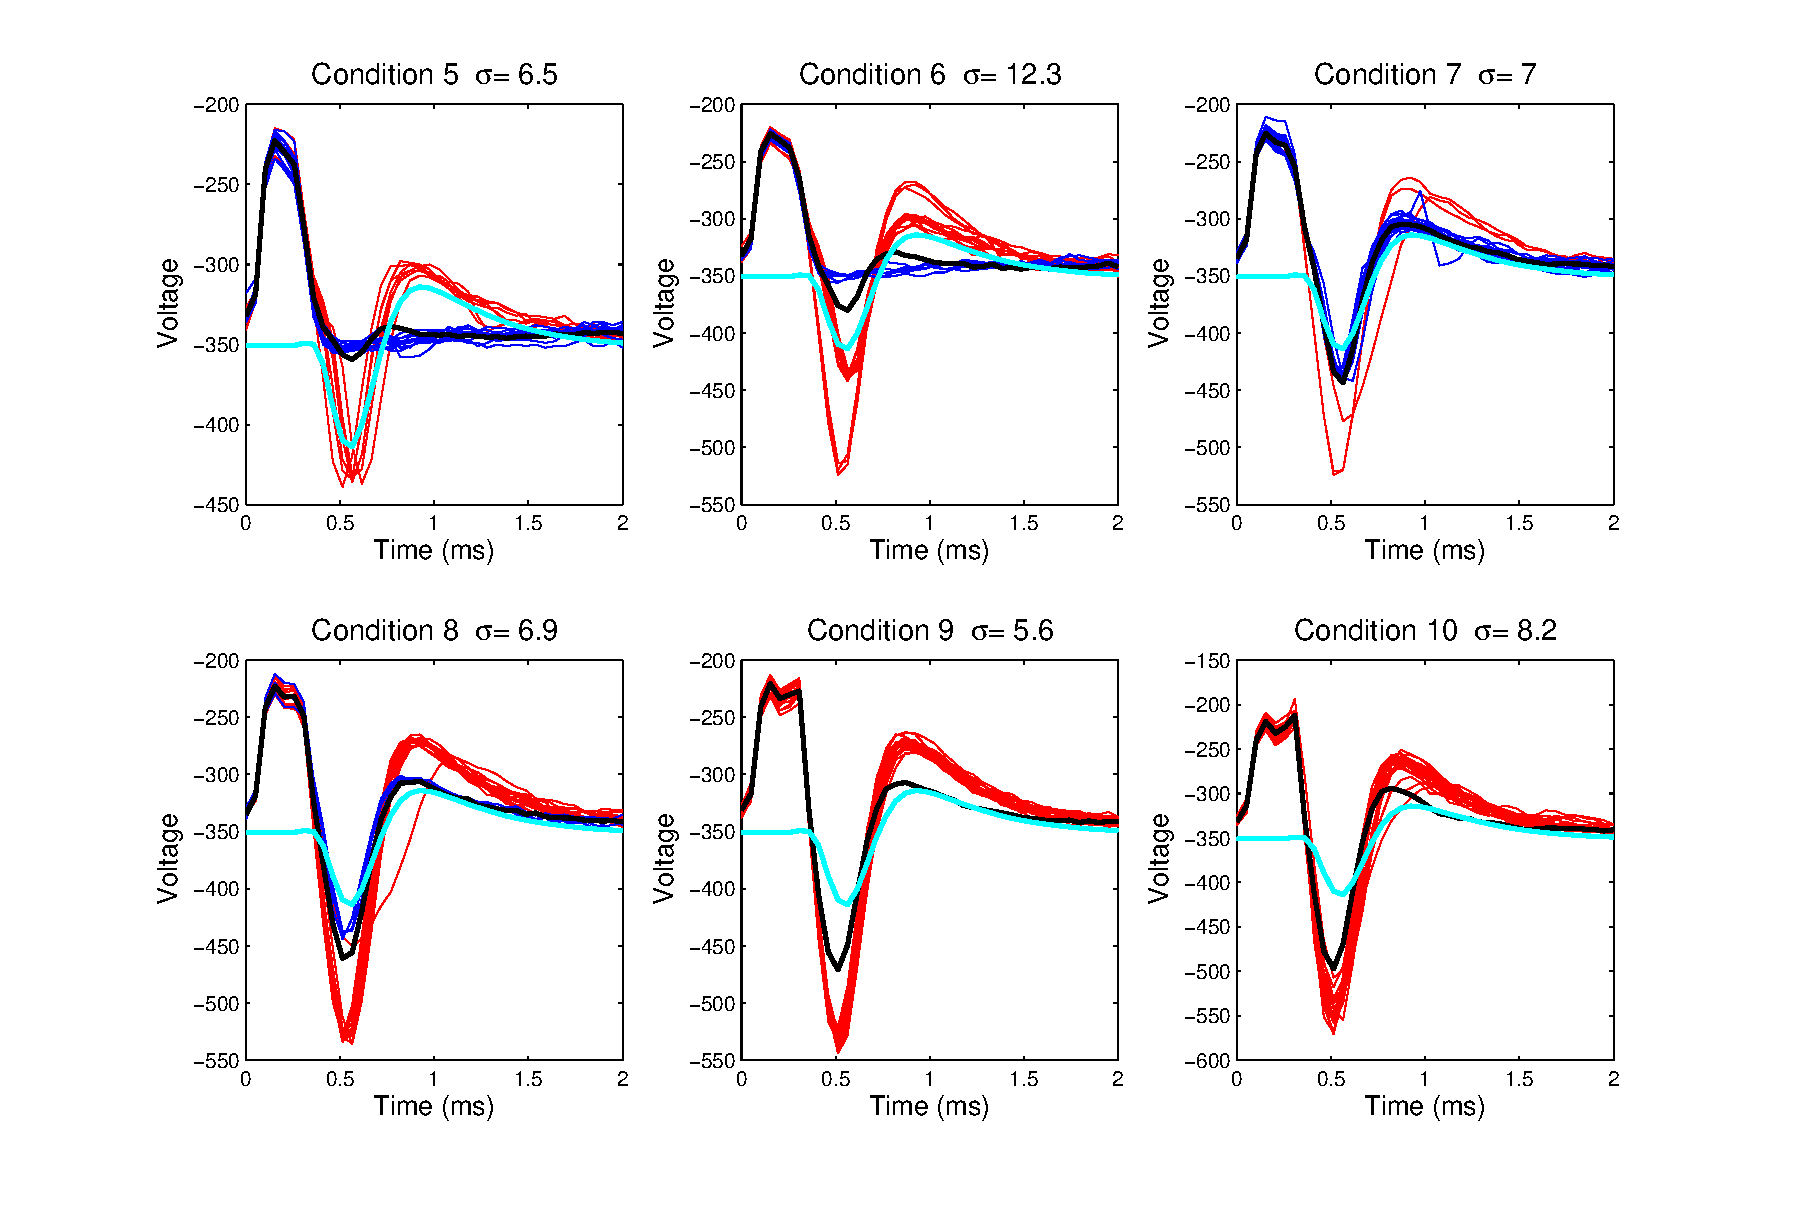
\includegraphics[height=4in]{TracesEl170pattern1443.eps}
   \caption{Traces}
                \label{fig:gull}
        \end{subfigure}% 
\centering

\begin{subfigure}[b]{\textwidth}
                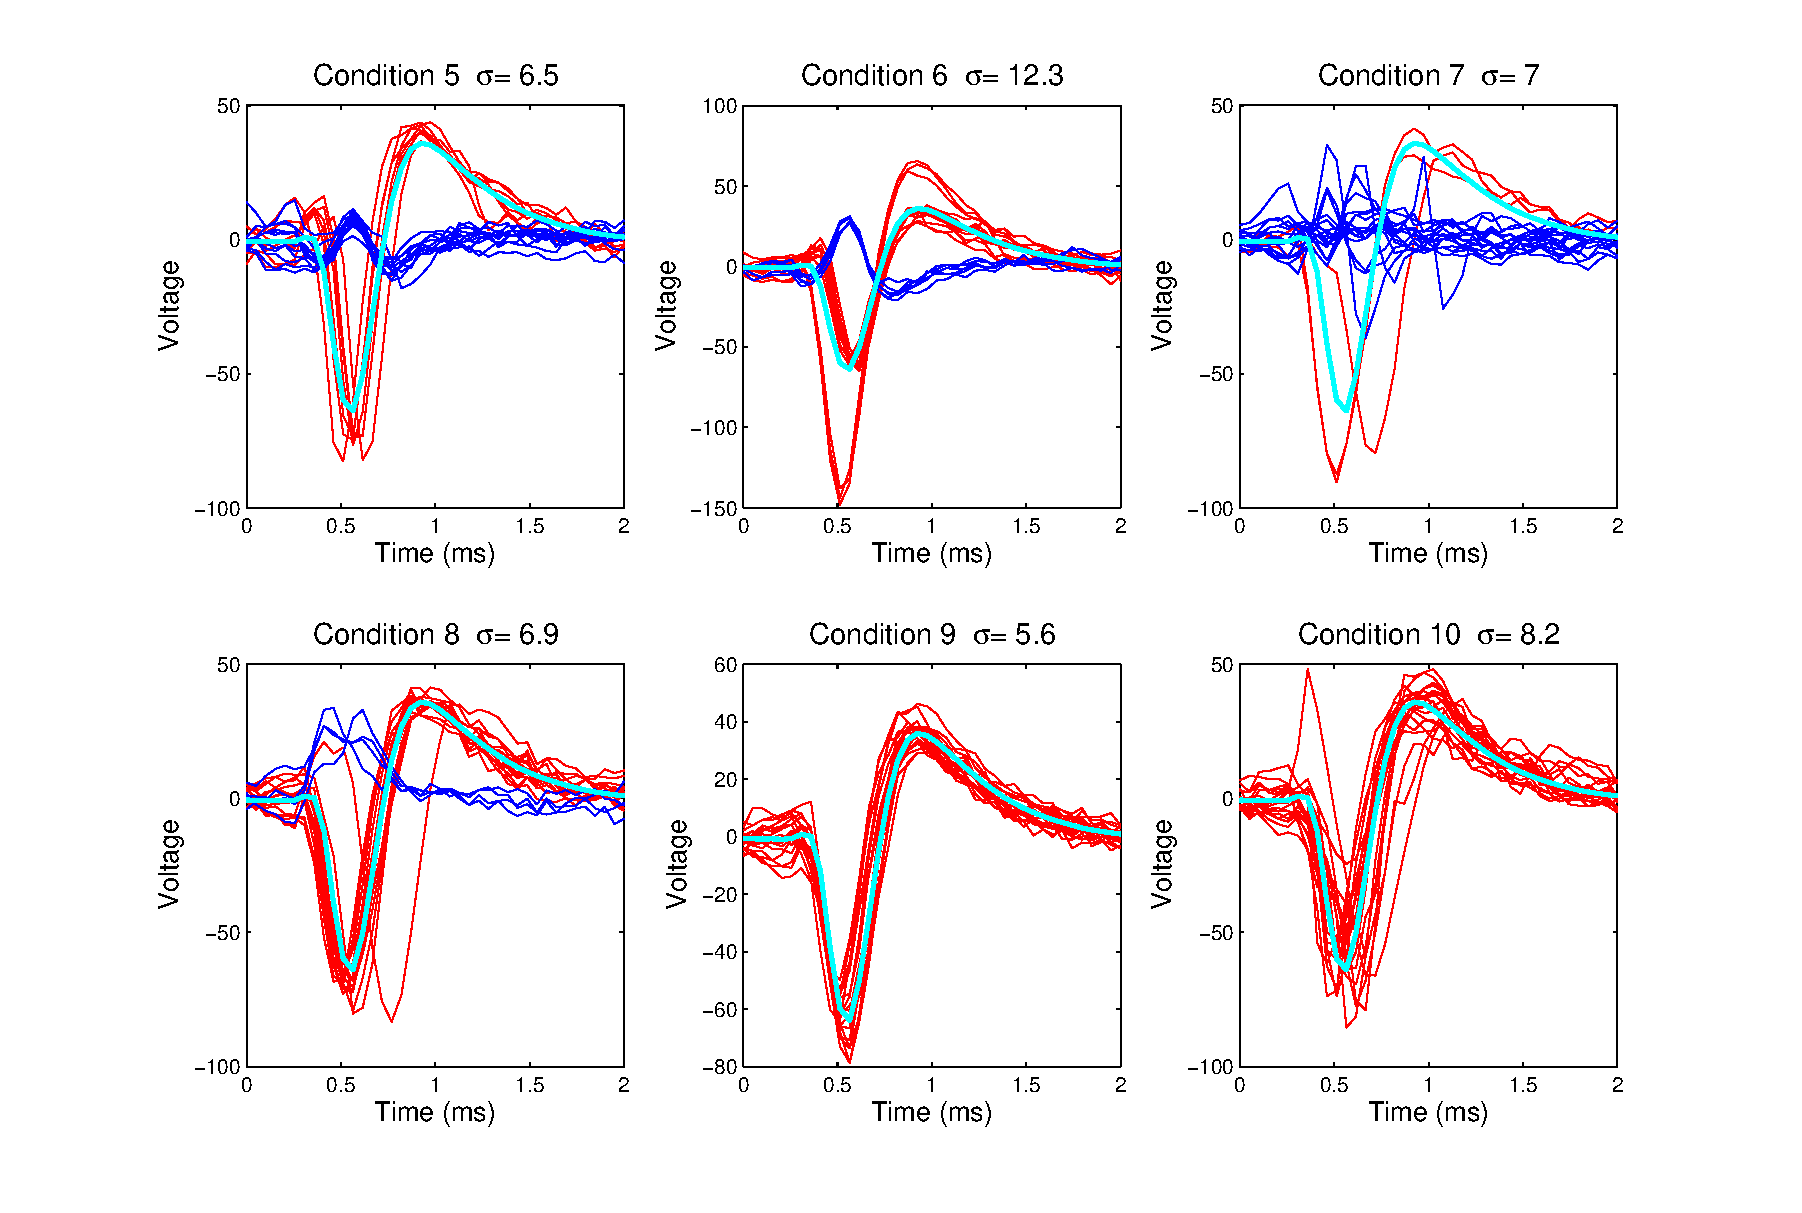
\includegraphics[height=4in]{ResidualsEl170pattern1443.eps}
                \label{fig:tiger}
                \caption{Artifact substracted residuals}
        \end{subfigure}
\caption{An example of failure in detection with axonal activation. Cyan trace: spike template, blue traces: trials with no spike, red traces: trials with spikes, black: artifact estimate}
\end{figure}

 \bibliographystyle{unsrt} 
\bibliography{references}


    \end{document}
